\documentclass[12pt]{article}

\usepackage[top=1in,bottom=1in,left=1in,right=1in]{geometry}
\usepackage{amsmath,amssymb,mathtools}
\usepackage{xcolor}
\usepackage{graphicx}
\usepackage{hyperref}
\usepackage{enumitem}

\hypersetup{
    pdfauthor={},
    pdftitle={MATH 1075 - Lesson 6.1 Recitation}
}

\begin{document}

\begin{center}
    {\LARGE MATH 1075 - Section 10.7 Worksheet}

    \vspace{2em}

    {\large 11/19/2026}
\end{center}

\section{Solving Radical Equations}
\begin{figure}[htbp]
    \centering
    % Replace "my_image" with your actual file name (without extension)
    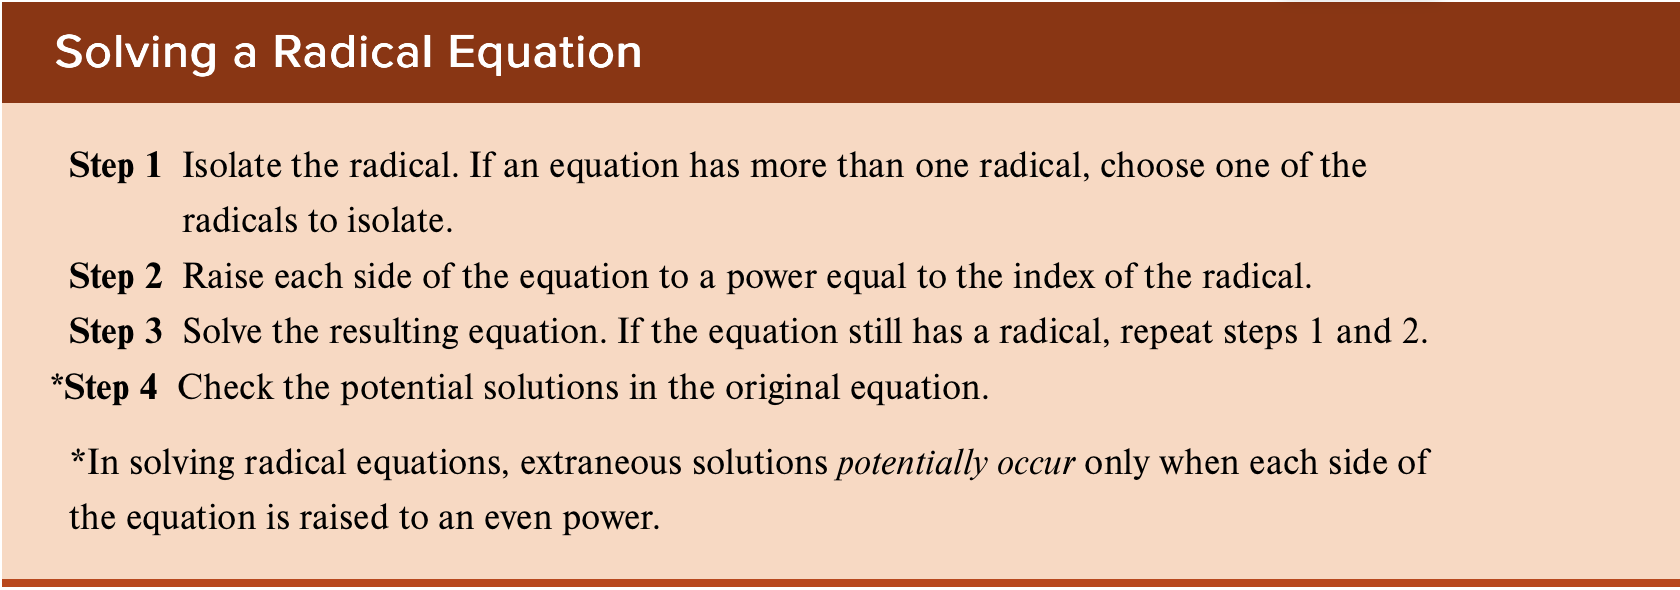
\includegraphics[width=1\linewidth]{Screenshot 2026-11-17 at 11.07.33 AM.png} 
\end{figure}
Solve the following radical equations. 

\vspace{1.5em}

1. $\sqrt{x+1}=5$

\vspace{6.5em} 

2. $\sqrt{x}=-7$

\vspace{6.5em} 

3. $\sqrt[4]{x}+2=8$

\vspace{6.5em} 

4. $\sqrt[3]{5y+1}=4$

\vspace{6.5em}

5. $\sqrt{x^{2}+5}=x+1$ 

\vspace{6.5em}


6. $\sqrt[4]{3b+6}=\sqrt[4]{7b-6}$ 

\vspace{6.5em} 

7. $\sqrt{5a-9}=\sqrt{5a}-3$ 

\vspace{6.5em} 

8. $\sqrt{p+7}-\sqrt{2p}-1=0$ 

\vspace{6.5em} 

\section{Applications of Radical Equations} 

\vspace{1.5em} 
If an object is dropped from an initial height $h$, its velocity at impact with the ground is given by
$$v = \sqrt{2gh}$$
where $g$ is the acceleration due to gravity and h is the initial height.\\

\noindent a. Find the initial height (in feet) of an object if its velocity at impact is 44 ft/sec. (Assume that the acceleration due to gravity is $g = 32 ft/sec^{2} $.)

\vspace{10em}

\noindent b. Find the initial height (in meters) of an object if its velocity at impact is 26 m/sec. (Assume that the acceleration due to gravity is $g = 9.8 m/sec^{2}$.) Round to the nearest tenth of a meter.

\end{document}